\chapter{Podstawowe pojęcia}\label{chap:pojecia}
W tym rozdziale zostaną przybliżone podstawowe pojęcia związane
z geometrią obliczeniową i problemami dotyczącymi wielokątów
wypukłych.

\begin{definicja}
  \emph{Wielokątem prostym} nazywamy taki wielokąt, że jedyne punkty
  płaszczyzny należące jednocześnie do dwóch jego krawędzi są jego
  wierzchołkami.
\end{definicja}

\begin{definicja}
  \emph{Wielokątem wypukłym} nazywamy wielokąt prosty którego wnętrze
  jest \emph{zbiorem wypukłym}, tzn.\ wszystkie punkty należące do
  odcinka łączącego dwa dowolne punkty ze zbioru należą do tego
  zbioru.
\end{definicja}

% brzeg wielokąta, wnętrze i zewnętrze wielokąta
% rysunki !

\begin{figure}[htb]
  \centering
  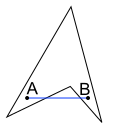
\includegraphics{img/nonconvex}
  \caption{Przykład czworokąta, który nie jest wypukły.}
\end{figure}

\begin{definicja}
  \emph{Średnicą zbioru punktów} nazywamy największą odległość
  pomiędzy dwoma punktami należącymi do tego zbioru.
\end{definicja}

\begin{definicja}
  Niech $p_{1}=(x_{1},y_{1})$, $p_{2}=(x_{2},y_{2})$,
  $p_{3}=(x_{3},y_{3})$ będą punktami na płaszczyźnie
  $\mathbb{R}^2$. \emph{Wyznacznikiem} współrzędnych tych punktów
  nazywamy liczbę

  \begin{center}
    \begin{math}
      X(p_1, p_2, p_3) =
      \begin{vmatrix}
        x_1 & y_1 & 1 \\
        x_2 & y_2 & 1 \\
        x_3 & y_3 & 1
      \end{vmatrix}
      .
    \end{math}
  \end{center}

  Kąt $\angle p_{1}p_{2}p_{3}$ nazywamy \emph{lewoskrętnym}, jeżeli
  wyznacznik $X(p_1, p_2, p_3)$ jest dodatni, w przeciwnym przypadku
  mówimy, że kąt ten jest \emph{prawoskrętny}.
\end{definicja}

\begin{definicja}
  \emph{Prostymi wspierającymi} dla wielokąta nazywamy takie proste,
  które przechodząc przez wierzchołek wielkąta nie przecinają jego
  wnętrza.
\end{definicja}

\begin{definicja}
  Mówimy, że para wierzchołków tworzy \emph{punkty antypodyczne},
  jeżeli można poprowadzić przez te wierzchołki przynajmniej dwie
  różne równoległe proste wspierające.
\end{definicja}

\begin{definicja}\label{def:bigo}
  Mówimy, że funkcja $f\colon \mathbb{N} \to \mathbb{R}$ jest co
  najwyżej rzędu $g$ (jest \emph{ograniczona} przez funkcję $g\colon
  \mathbb{N} \to \mathbb{R}$), gdy istnieją takie stałe $n_0 > 0$ oraz
  $c > 0$, że

  \begin{center}
    $\forall n \geq n_0\ f(n) \leq c \cdot g(n)$.
  \end{center}
\end{definicja}

W niniejszej pracy do opisu wydajności algorytmów będziemy korzystać z
\emph{notacji wielkiego O}. Jest to notacja asymptotycznego tempa
wzrostu wartości funkcji względem jej argumentów, w algorytmice
stosowana do charakterystyki złożoności obliczeniowej algorytmów
opisując ilość potrzebnych zasobów (czasu lub pamięci) w stosunku do
rozmiaru danych wejściowych. Zgodnie z tą notacją złożoność czasową
algorytmu o czasie działania $T(n) = f(n)$, gdzie $f(n)$ spełnia
definicję~\ref{def:bigo}, zapisalibyśmy jako $T(n) = O(g(n))$.

\begin{table}[htb]
  \centering

  \begin{tabular}{ll}
    \toprule
    $O(1)$ & stała \\
    \midrule
    $O(\log n)$ & logarytmiczna \\
    \midrule
    $O(n)$ & liniowa \\
    \midrule
    $O(n \log n)$ & liniowo-logarytmiczna \\
    \midrule
    $O(n^2)$ & kwadratowa \\
    \midrule
    $O(n^c)$ & wielomianowa \\
    \midrule
    $O(c^n)$ & wykładnicza $(c > 1)$ \\
    \midrule
    $O(n!)$ & ograniczona przez silnię \\
    \bottomrule
  \end{tabular}

  \caption{Najczęściej wyróżniane rzędy złożoności obliczeniowej,
    podane według rosnącej złożoności.}
\end{table}

W tej pracy \emph{efektywnym} algorytmem dla wielokąta wypukłego
będziemy nazywać algorytm o mniejszej złożoności obliczeniowej niż
najlepszy znany algorytm dla wielokąta prostego dla tego samego
problemu.

% przyjęte oznaczenia

%%% Local Variables:
%%% mode: latex
%%% TeX-master: "masterthesis"
%%% TeX-engine: xetex
%%% End:
